\documentclass{beamer}
\usepackage{tikz}
\usepackage{xcolor}

\definecolor{darkgreen}{rgb}{0.0, 0.7, 0.13}
\setbeamertemplate{navigation symbols}{}%remove navigation symbols

\begin{document}

\begin{frame}
%\frametitle{Nonidentifiability in the relaxed clock}

\begin{columns}
\column{0.38\textwidth}
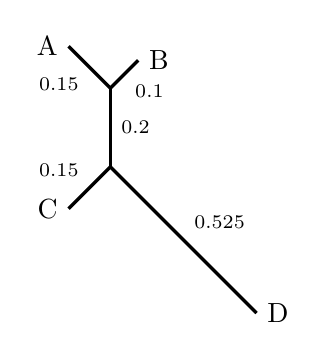
\begin{tikzpicture}[scale=0.5,rotate=-90]
%  \node[anchor=north, line width=1.25pt] at (236.66667pt, 116.66666pt) {B};
%  \node[anchor=north, line width=1.25pt] at (190pt, 132.22223pt) {A};
%  \draw[line width=1.25pt] (236.66667pt, 116.66667pt) -- node[auto] {\scriptsize{0.1}} (236.66667pt, 85.55556pt) -- (213.33333pt, 85.55556pt);
%  \draw[line width=1.25pt] (190pt, 132.22222pt) --  node[auto] {\scriptsize{0.15}} (190pt, 85.55556pt) -- (213.33333pt, 85.55556pt);
%  \node[anchor=north, line width=1.25pt] at (283.33334pt, 70pt) {C};
%  \draw[line width=1.25pt] (213.33333pt, 85.55556pt) -- node[auto] {\scriptsize{0.2}} (213.33333pt, 23.33333pt) -- (248.33333pt, 23.33333pt);
%  \draw[line width=1.25pt] (283.33333pt, 70pt) -- node[auto] {\scriptsize{0.15}} (283.33333pt, 23.33333pt) -- (248.33333pt, 23.33333pt);
%  \node[anchor=north, line width=1.25pt] at (330pt, 140pt) {D};
%  \draw[line width=1.25pt] (248.33333pt, 23.33333pt) -- node[auto] {\scriptsize{0.075}} (248.33333pt, 0pt) -- (289.16667pt, 0pt);
%  \draw[line width=1.25pt] (330pt, 140pt) -- node[auto] {\scriptsize{0.45}} (330pt, 0pt) -- (289.16667pt, 0pt);
  
   \draw[line width=1.25pt] (2,2)  -- node[auto] {\scriptsize{0.2}} (4,2);
  \draw[line width=1.25pt] (2,2) -- node[auto] {\scriptsize{0.15}} (0.9393398,0.9393398);
  \node[anchor=east, line width=1.25pt] at (0.9393398,0.9393398) {A};
  \draw[line width=1.25pt] (2,2) -- node[auto,swap] {\scriptsize{0.1}} (1.292893,2.707107);
  \node[anchor=west, line width=1.25pt] at (1.292893,2.707107) {B};

  \draw[line width=1.25pt] (4,2) -- node[auto,swap] {\scriptsize{0.15}} (5.06066,0.9393398);
  \node[anchor=east, line width=1.25pt] at (5.06066,0.9393398) {C};
  \draw[line width=1.25pt] (4,2) -- node[auto] {\scriptsize{0.525}} (7.712311,5.712311);
  \node[anchor=west, line width=1.25pt] at (7.712311,5.712311) {D};

  
\end{tikzpicture}
\column{0.24\textwidth}

$=\textcolor{darkgreen}{\begin{pmatrix}0.015\\0.01\\0.005\\0.01\\0.01\\0.005\end{pmatrix}}\star$

\column{0.38\textwidth}
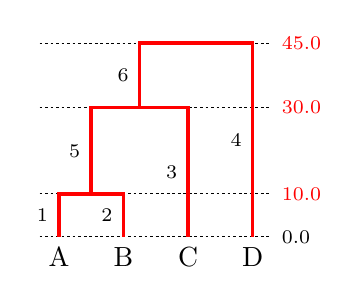
\begin{tikzpicture}[yscale=-0.50,xscale=0.50]
  \draw[dash pattern=on 1.0 off 1.0 ] (-14pt, 140pt) -- (154pt, 140pt);
  \node[anchor=west, dash pattern=on 1.0 off 1.0 ] at (154pt, 140pt) {\scriptsize{0.0}};
  \draw[dash pattern=on 1.0 off 1.0 ] (-14pt, 108.88889pt) -- (154pt, 108.88889pt);
  \node[red,anchor=west, dash pattern=on 1.0 off 1.0 ] at (154pt, 108.88889pt) {\scriptsize{10.0}};
  \draw[dash pattern=on 1.0 off 1.0 ] (-14pt, 46.66667pt) -- (154pt, 46.66667pt);
  \node[red,anchor=west, dash pattern=on 1.0 off 1.0 ] at (154pt, 46.66667pt) {\scriptsize{30.0}};
  \draw[dash pattern=on 1.0 off 1.0 ] (-14pt, 0pt) -- (154pt, 0pt);
  \node[red,anchor=west, dash pattern=on 1.0 off 1.0 ] at (154pt, 0pt) {\scriptsize{45.0}};
  \node[anchor=north, line width=1.25pt] at (0pt, 140pt) {A};
  \node[anchor=north, line width=1.25pt] at (46.66667pt, 140pt) {B};
  \draw[line width=1.25pt,red] (0pt, 140pt) -- (0pt, 108.88889pt) -- (23.33333pt, 108.88889pt);
  \node[anchor=east, line width=1.25pt] at (0pt, 124.44444pt) {\scriptsize{1}};
  \draw[line width=1.25pt,red] (46.66667pt, 140pt) -- (46.66667pt, 108.88889pt) -- (23.33333pt, 108.88889pt);
  \node[anchor=east, line width=1.25pt] at (46.66667pt, 124.44444pt) {\scriptsize{2}};
  \node[anchor=north, line width=1.25pt] at (93.33334pt, 140pt) {C};
  \draw[line width=1.25pt,red] (23.33333pt, 108.88889pt) -- (23.33333pt, 46.66667pt) -- (58.33333pt, 46.66667pt);
  \node[anchor=east, line width=1.25pt] at (23.33333pt, 77.77778pt) {\scriptsize{5}};
  \draw[line width=1.25pt,red] (93.33333pt, 140pt) -- (93.33333pt, 46.66667pt) -- (58.33333pt, 46.66667pt);
  \node[anchor=east, line width=1.25pt] at (93.33334pt, 93.33334pt) {\scriptsize{3}};
  \node[anchor=north, line width=1.25pt] at (140pt, 140pt) {D};
  \draw[line width=1.25pt,red] (58.33333pt, 46.66667pt) -- (58.33333pt, 0pt) -- (99.16667pt, 0pt);
  \node[anchor=east, line width=1.25pt] at (58.33333pt, 23.33333pt) {\scriptsize{6}};
  \draw[line width=1.25pt,red] (140pt, 140pt) -- (140pt, 0pt) -- (99.16667pt, 0pt);
  \node[anchor=east, line width=1.25pt] at (140pt, 70pt) {\scriptsize{4}};
\end{tikzpicture}

\end{columns}

\begin{columns}
\column{0.38\textwidth}
\column{0.24\textwidth}


$=\textcolor{darkgreen}{\begin{pmatrix}\mathbf{0.0075}\\\mathbf{0.005}\\0.005\\0.01\\\mathbf{0.02}\\0.005\end{pmatrix}}\star$

\column{0.38\textwidth}
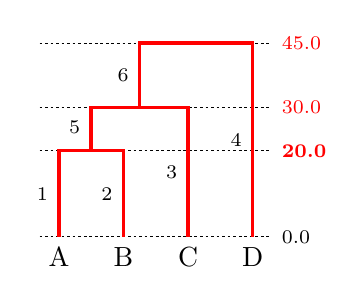
\begin{tikzpicture}[yscale=-0.50,xscale=0.50]
  \draw[dash pattern=on 1.0 off 1.0 ] (-14pt, 140pt) -- (154pt, 140pt);
  \node[anchor=west, dash pattern=on 1.0 off 1.0 ] at (154pt, 140pt) {\scriptsize{0.0}};
  \draw[dash pattern=on 1.0 off 1.0 ] (-14pt, 77.77777pt) -- (154pt, 77.77777pt);
  \node[red,anchor=west, dash pattern=on 1.0 off 1.0 ] at (154pt, 77.77777pt) {\scriptsize{\bf20.0}};
  \draw[dash pattern=on 1.0 off 1.0 ] (-14pt, 46.66667pt) -- (154pt, 46.66667pt);
  \node[red,anchor=west, dash pattern=on 1.0 off 1.0 ] at (154pt, 46.66667pt) {\scriptsize{30.0}};
  \draw[dash pattern=on 1.0 off 1.0 ] (-14pt, 0pt) -- (154pt, 0pt);
  \node[red,anchor=west, dash pattern=on 1.0 off 1.0 ] at (154pt, 0pt) {\scriptsize{45.0}};
  \node[anchor=north, line width=1.25pt] at (0pt, 140pt) {A};
  \node[anchor=north, line width=1.25pt] at (46.66667pt, 140pt) {B};
  \draw[line width=1.25pt,red] (0pt, 140pt) -- (0pt, 77.77777pt) -- (23.33333pt, 77.77777pt);
  \node[anchor=east, line width=1.25pt] at (0pt, 108.88888pt) {\scriptsize{1}};
  \draw[line width=1.25pt,red] (46.66667pt, 140pt) -- (46.66667pt, 77.77777pt) -- (23.33333pt, 77.77777pt);
  \node[anchor=east, line width=1.25pt] at (46.66667pt, 108.88888pt) {\scriptsize{2}};
  \node[anchor=north, line width=1.25pt] at (93.33334pt, 140pt) {C};
  \draw[line width=1.25pt,red] (23.33333pt, 77.77777pt) -- (23.33333pt, 46.66667pt) -- (58.33333pt, 46.66667pt);
  \node[anchor=east, line width=1.25pt] at (23.33333pt, 61pt) {\scriptsize{5}};
  \draw[line width=1.25pt,red] (93.33333pt, 140pt) -- (93.33333pt, 46.66667pt) -- (58.33333pt, 46.66667pt);
  \node[anchor=east, line width=1.25pt] at (93.33334pt, 93.33334pt) {\scriptsize{3}};
  \node[anchor=north, line width=1.25pt] at (140pt, 140pt) {D};
  \draw[line width=1.25pt,red] (58.33333pt, 46.66667pt) -- (58.33333pt, 0pt) -- (99.16667pt, 0pt);
  \node[anchor=east, line width=1.25pt] at (58.33333pt, 23.33333pt) {\scriptsize{6}};
  \draw[line width=1.25pt,red] (140pt, 140pt) -- (140pt, 0pt) -- (99.16667pt, 0pt);
  \node[anchor=east, line width=1.25pt] at (140pt, 70pt) {\scriptsize{4}};
\end{tikzpicture}

\end{columns}


\bigskip{}

\begin{columns}
\column{0.33\textwidth}
\centering
``substitution tree''
\column{0.33\textwidth}
\centering
evolutionary rates
\scriptsize{substitutions / site / unit time}
\column{0.33\textwidth}
\centering
time tree
\end{columns}
\end{frame}
\end{document}